\newpage
	\section{Цель и задачи работы}
		\textbf{Цель работы}: приобретение практических навыков реализации важнейших элементов лексических анализаторовна
			примере распознавания цепочек регулярного языка.\\

		\textbf{Задачи работы:}
		\begin{enumerate}
			\item Ознакомиться с основными понятиями и определениями, лежащими в основе построения лексических анализаторов.
			\item Прояснить связь между регулярным множеством, регулярным выражением, праволинейным языком,
				конечно-автоматным языком и недетерминированным конечно-автоматным языком.
			\item Разработать, тестировать и отладить программу распознавания цепочек регулярного или
				праволинейного языка в соответствии с предложенным вариантом грамматики.
		\end{enumerate}


%%%%%%%%%%%%%%%%%%%%%%%%%%%%%%
	\section{Листинг}
        
        \lstset{inputencoding=utf8x, extendedchars=\true, breaklines=true, numbers=left,
        keywordstyle=\color{blue}, commentstyle=\color{red}}
        
        \subsection{main.py}
        \lstinputlisting[language=python]{../../main.py}

        \subsection{regexp\_process.py}
        \lstinputlisting[language=python]{../../regexp_process.py}

        \subsection{FSM.py}
        \lstinputlisting[language=python]{../../FSM.py}

        \subsection{utils.py}
        \lstinputlisting[language=python]{../../utils.py}

% 		\begin{lstlisting}[caption=main.py]
% from tabulate import tabulate
% from utils import format_table_for_tabulate_dka, format_table_for_tabulate_nka
% from regexp_process import get_postfix_regexp, TEST_ALPHABET, ALL_TEST_SYMBOLS, RegexpError
% from FSM import generate_nfsm_from_pregexp, draw_nka_gz, \
%     generate_dfsm_from_nfsm, draw_dka_gz, \
%     generate_min_dka_from_dka, \
%     generate_min_dka_from_pregexp, \
%     dka_job

% # TEST_REGEXP = 'ab|baba(abb*)+'
% # TEST_REGEXP = '(b|ab*ab*)*'
% # TEST_REGEXP = '(ab)*|ba'
% # TEST_REGEXP = '(a|b)*abb'
% # TEST_REGEXP = 'a|b|c'
% # TEST_REGEXP = 'ab'
% # TEST_REGEXP = 'a*'


% if __name__ == '__main__':
%     TEST_REGEXP = input('Введите выражение, для которого необходимо построить автомат: ')
%     if [x for x in TEST_REGEXP if x not in ALL_TEST_SYMBOLS]:
%         print('Выражение не соответствует допустимому алфавиту')
%         exit(1)

%     postfix_regexp = ''
%     try:
%         postfix_regexp = get_postfix_regexp(TEST_REGEXP)
%         print(f'Постфиксная запись регулярного выражения: {"".join(postfix_regexp)}')
%     except RegexpError as e:
%         print(e)
%         exit(1)

%     nka = generate_nfsm_from_pregexp(postfix_regexp, TEST_ALPHABET)
%     table, headers = format_table_for_tabulate_nka(nka.get_as_table(TEST_ALPHABET), TEST_ALPHABET)
%     print('\nНКА:')
%     print(tabulate(table, headers=headers))
%     draw_nka_gz(nka)

%     dka = generate_dfsm_from_nfsm(nka.get_as_table(TEST_ALPHABET), TEST_ALPHABET)
%     table, headers = format_table_for_tabulate_dka(dka, TEST_ALPHABET)
%     print('\nДКА:')
%     print(tabulate(table, headers=headers))
%     draw_dka_gz(dka)

%     min_dka = generate_min_dka_from_dka(dka, TEST_ALPHABET)
%     table, headers = format_table_for_tabulate_dka(min_dka, TEST_ALPHABET)
%     print('\nМинимальный ДКА:')
%     print(tabulate(table, headers=headers))
%     draw_dka_gz(min_dka, is_min=True)

%     to_check = ''
%     while to_check != '$':
%         to_check = input('\nВведите слово, которое нужно проверить ($ для завершения): ')
%         try:
%             is_ok = dka_job(min_dka, to_check)
%         except ValueError as e:
%             if to_check == '$':
%                 break
%             print(e)
%             continue
%         if is_ok:
%             print('Автомат допускает введенное слово')
%         else:
%             print('Автомат не допускает введенное слово')

%     print('Пока-пока :)')
            
% 		\end{lstlisting}

% 		\begin{lstlisting}[caption=regexp_process.py]
% from typing import List


% # TEST_ALPHABET = [chr(x) for x in range(ord('a'), ord('z')+1)] + [chr(x) for x in range(ord('A'), ord('Z')+1)] + \
% #                 [str(x) for x in range(10)]
% TEST_ALPHABET = ['a', 'b']
% TEST_OPS_PRECEDENCE = {
%     '|': 0,
%     '+': 2,
%     '*': 2,
%     '(': -1,
%     ')': -1,
%     '.': 1,
% }
% TEST_OPS = list(TEST_OPS_PRECEDENCE.keys())
% ALL_TEST_SYMBOLS = TEST_ALPHABET + TEST_OPS
% CONCAT_OP = TEST_OPS[-1]


% class RegexpError(Exception):
%     def __init__(self, message: str):
%         self.message = message

%     def __str__(self):
%         return self.message


% def get_postfix_regexp(regexp: str) -> List[str]:
%     return __create_postfix_notation_regexp(__normalize_regexp(regexp))


% def __normalize_regexp(regexp: str) -> str:
%     """
%     Добавление знака конкатенации к регулярке
%     :param regexp: Регулярка
%     :return: Регулярка со знаками конкатенации
%     """
%     nregexp = ''
%     for i in range(len(regexp)-1):
%         if regexp[i] not in ALL_TEST_SYMBOLS:
%             raise RegexpError(message=f'Неизвестный символ "{regexp[i]}"')
%         nregexp += regexp[i]
%         if regexp[i] in TEST_ALPHABET + ['*', '+', ')'] and regexp[i+1] in TEST_ALPHABET + ['(']:
%             nregexp += CONCAT_OP
%     if regexp[-1] not in ALL_TEST_SYMBOLS:
%         raise RegexpError(message=f'Неизвестный символ "{regexp[-1]}"')
%     nregexp += regexp[-1]
%     return nregexp


% def __create_postfix_notation_regexp(normalized_regexp: str) -> List[str]:
%     """
%     Перевод регекспа из инфиксной записи в постфиксную
%     :param normalized_regexp: Регулярка с символами конкатенации
%     :return: Постфиксная нотация регекспа
%     """
%     queue = []
%     stack = []
%     while len(normalized_regexp) != 0:
%         sym = normalized_regexp[0]
%         normalized_regexp = normalized_regexp[1:]
%         if sym in TEST_ALPHABET:
%             queue.append(sym)
%         elif sym == '(':
%             stack.append('(')
%         elif sym == ')':
%             while len(stack) > 0 and stack[-1] != '(':
%                 queue.append(stack.pop())
%             try:
%                 stack.pop()
%             except IndexError:
%                 raise RegexpError('Не хватает открывающей скобки')
%         elif sym in TEST_OPS:
%             while len(stack) > 0 and TEST_OPS_PRECEDENCE[stack[-1]] >= TEST_OPS_PRECEDENCE[sym]:
%                 queue.append(stack.pop())
%             stack.append(sym)
%         else:
%             raise RegexpError('Неизвестный символ в построении постфиксной формы')
%     while len(stack) > 0:
%         stack_sym = stack.pop()
%         if stack_sym == '(':
%             raise RegexpError('Не хватает закрывающей скобки')
%         queue.append(stack_sym)
%     return queue
            
% 		\end{lstlisting}

% 		\begin{lstlisting}[caption=FSM.py]
% from typing import List, Dict, Set, Tuple, Iterable, Union
% from graphviz import Digraph


% # MARK: - NFMS

% class FiniteStateMachineNode:
%     """
%     Состояние конечного автомата
%     outputs в формате [(node1, <символ перехода>), ...]
%     """

%     def __init__(self, state, outputs=None):
%         if outputs is None:
%             outputs = list()
%         self.state = state
%         self.outputs = outputs

%     @property
%     def is_end_state(self):
%         return len(self.outputs) == 0

%     def outputs_append(self, node, symbol='eps'):
%         self.outputs.append((node, symbol))

%     def __str__(self):
%         return str(self.state)

%     def __repr__(self):
%         return str(self)


% class NKA:
%     """
%     Класс для НКА
%     """
%     state_num = 0

%     def __init__(self, root_state: FiniteStateMachineNode = None, symbol: str = 'eps'):
%         if root_state:
%             self.root_state = root_state
%         else:
%             st_node = FiniteStateMachineNode(state=NKA.state_num + 1)
%             end_node = FiniteStateMachineNode(state=NKA.state_num + 2)
%             st_node.outputs_append(end_node, symbol=symbol)
%             self.root_state = st_node
%             NKA.state_num += 2

%     def copy(self):
%         return NKA(self.root_state)

%     @property
%     def end_state(self):
%         node = self.root_state
%         while not node.is_end_state:
%             node = node.outputs[0][0]
%         return node

%     def concat(self, nka):
%         """
%         (self) -eps-> (nka)
%         """
%         onode_1, onode_2 = self.copy(), nka.copy()
%         onode_1.end_state.outputs_append(onode_2.root_state)
%         return NKA(root_state=onode_1.root_state)

%     def oorr(self, nka):
%         """
%             //eps->(self)-\
%         (S)-|             |-eps->(F)
%             \\eps->(nka)-/

%         """
%         st_node = FiniteStateMachineNode(state=NKA.state_num + 1)
%         end_node = FiniteStateMachineNode(state=NKA.state_num + 2)
%         onode_1, onode_2 = self.copy(), nka.copy()
%         onode_1.end_state.outputs_append(end_node)
%         onode_2.end_state.outputs_append(end_node)
%         st_node.outputs_append(onode_1.root_state)
%         st_node.outputs_append(onode_2.root_state)
%         NKA.state_num += 2
%         return NKA(root_state=st_node)

%     def plus(self):
%         """
%             /<--------eps---------\
%         (S) -eps-> (self) -eps-> (PF) -eps-> (F)
%         """
%         st_node = FiniteStateMachineNode(state=NKA.state_num + 1)
%         pre_end_node = FiniteStateMachineNode(state=NKA.state_num + 2)
%         end_node = FiniteStateMachineNode(state=NKA.state_num + 3)
%         onode = self.copy()
%         pre_end_node.outputs_append(end_node)
%         pre_end_node.outputs_append(st_node)
%         onode.end_state.outputs_append(pre_end_node)
%         st_node.outputs_append(onode.root_state)
%         NKA.state_num += 3
%         return NKA(root_state=st_node)

%     def star(self):
%         """
%             /<--------eps---------\
%         (S) -eps-> (self) -eps-> (PF) -eps-> (F)
%             \\--------eps-------->/
%         """
%         st_node = FiniteStateMachineNode(state=NKA.state_num + 1)
%         pre_end_node = FiniteStateMachineNode(state=NKA.state_num + 2)
%         end_node = FiniteStateMachineNode(state=NKA.state_num + 3)
%         onode = self.copy()
%         pre_end_node.outputs_append(end_node)
%         pre_end_node.outputs_append(st_node)
%         onode.end_state.outputs_append(pre_end_node)
%         st_node.outputs_append(end_node)
%         st_node.outputs_append(onode.root_state)
%         NKA.state_num += 3
%         return NKA(root_state=st_node)

%     def __get_table_row(self, alphabet: List[str]) -> Dict[str, List[str]]:
%         ans = {'eps': []}
%         for sym in alphabet:
%             ans[sym] = []
%         return ans

%     def get_as_table(self, alphabet: List[str]) -> Dict[str, Dict[str, List[str]]]:
%         """
%         Автомат в виде таблицы
%         """
%         ans = {}
%         already_seen = []
%         stack = [self.root_state]
%         while len(stack) > 0:
%             node = stack.pop()
%             if str(node.state) in already_seen:
%                 continue
%             already_seen.append(str(node.state))
%             for nd, sym in node.outputs:
%                 stack.append(nd)
%                 try:
%                     row = ans[str(node.state)]
%                 except KeyError:
%                     ans[str(node.state)] = self.__get_table_row(alphabet)
%                     row = ans[str(node.state)]
%                 row[sym].append(str(nd.state))
%         ans['f'] = self.__get_table_row(alphabet)
%         return ans


% def generate_nfsm_from_pregexp(pregexp: List[str], alphabet: List) -> NKA:
%     """
%     Генерация НКА из постфиксной регулярки
%     :param alphabet: Допустимый алфавит
%     :param pregexp: Постфиксная регулярка
%     :return: Начальное состояние НКА
%     """
%     stack = []
%     while len(pregexp) > 0:
%         cur_symbol = pregexp.pop(0)
%         if cur_symbol in alphabet:
%             stack.append(NKA(symbol=cur_symbol))
%         elif cur_symbol == '.':
%             nka2 = stack.pop()
%             nka1 = stack.pop()
%             new_nka = nka1.concat(nka2)
%             stack.append(new_nka)
%         elif cur_symbol == '|':
%             nka2 = stack.pop()
%             nka1 = stack.pop()
%             new_nka = nka1.oorr(nka2)
%             stack.append(new_nka)
%         elif cur_symbol == '*':
%             nka = stack.pop()
%             new_nka = nka.star()
%             stack.append(new_nka)
%         elif cur_symbol == '+':
%             nka = stack.pop()
%             new_nka = nka.plus()
%             stack.append(new_nka)
%     start_node = FiniteStateMachineNode(state='s')
%     end_node = FiniteStateMachineNode(state='f')
%     nka = stack.pop()
%     nka.end_state.outputs_append(end_node)
%     start_node.outputs_append(nka.root_state)
%     return NKA(root_state=start_node)


% def draw_nka_gz(nka: NKA):
%     d = Digraph()
%     stack = [nka.root_state]
%     already_was = []
%     while len(stack) > 0:
%         node = stack.pop()
%         if node.state in already_was:
%             continue
%         already_was.append(node.state)
%         for tpl in node.outputs:
%             d.edge(f'{node.state}', f'{tpl[0].state}', label=tpl[1])
%             stack.append(tpl[0])
%     with open('nka', 'w') as f:
%         f.write(d.source)
%     d.render('nka', view=True)


% # MARK: - DFMS

% class DFSMState:
%     """
%     Класс для состояния ДКА
%     """

%     def __init__(self, state: str, nka_states: Set[str], outputs: List[Tuple[str, str]] = None, is_final=False):
%         """
%         :param state: Состояние
%         :param nka_states: Множество состояний НКА, соответствующих данному состоянию ДКА
%         :param outputs: Переходы в другие состояния в формате (state, symbol)
%         :param is_final: Является ли состояние финальным
%         """
%         self.state = state
%         self.nka_states = nka_states
%         self.outputs = outputs or []
%         self.is_final = is_final
%         if self.is_final:
%             self.state += 'f'

%     def append_output(self, state: str, symbol: str):
%         self.outputs.append((state, symbol))

%     def __str__(self):
%         return self.state

%     def __repr__(self):
%         return str(self)

%     def __eq__(self, other):
%         return self.nka_states == other.nka_states

%     def __hash__(self):
%         return hash(frozenset(self.nka_states))


% def generate_dfsm_from_nfsm(nfsm: Dict[str, Dict[str, List[str]]], alphabet: List[str]) -> List[DFSMState]:
%     """
%     Преобразование НКА (табличного представления) в ДКА (по сути тоже в табличное) по алгоритму из Ульмана
%     :param nfsm: НКА
%     :param alphabet: Допустимый алфавит
%     :return: ДКА
%     """
%     ans = []
%     __ec = __eps_closure_for_nka_state(nfsm, 's')
%     stack = [DFSMState('s', __ec, is_final='f' in __ec)]
%     marked_states = [(stack[0].nka_states, 's')]
%     states_cnt = 1
%     while len(stack) > 0:
%         dstate = stack.pop()
%         for asymbol in alphabet:
%             move_by_asymbol = __move_closure_for_set_of_nka_states(nfsm, dstate.nka_states, asymbol)
%             u = __eps_closure_for_set_of_nka_states(nfsm, move_by_asymbol)
%             new_dstate = DFSMState(state=str(states_cnt), nka_states=u, is_final='f' in u)
%             if new_dstate not in ans and new_dstate not in stack:
%                 stack.append(new_dstate)
%                 states_cnt += 1
%                 marked_states.append((new_dstate.nka_states, new_dstate.state))
%             dstate.append_output(state=[x[1] for x in marked_states if x[0] == u][0], symbol=asymbol)
%         ans.append(dstate)
%     return __remove_states_without_inputs(ans)


% def __remove_states_without_inputs(dka: List[DFSMState]) -> List[DFSMState]:
%     seen_in_output = {'s', 'sf'}
%     for state in dka:
%         for ostate, _ in state.outputs:
%             seen_in_output.add(ostate)
%     ans = []
%     for state in dka:
%         if state.state in seen_in_output:
%             ans.append(state)
%     return ans


% def __eps_closure_for_nka_state(nfsm, state: str) -> Set[str]:
%     """
%     Поиск эпсилон-замыкания из множества state
%     :param nfsm: НКА
%     :param state: Состояние
%     :return: Множество состояний, достижимых из данного только по eps-переходам
%     """
%     ans = {state}
%     stack = [state]
%     was_seen = []
%     while len(stack) > 0:
%         cur_state = stack.pop()
%         if cur_state in was_seen:
%             continue
%         was_seen.append(cur_state)
%         ans.add(state)
%         to_ext = nfsm[cur_state]['eps']
%         ans.update(to_ext)
%         stack.extend(to_ext)
%     return ans


% def __eps_closure_for_set_of_nka_states(nfsm, states) -> Set[str]:
%     """
%     Поиск эпсилон-замыкания из множества состояний states
%     :param nfsm: НКА
%     :param states: Состояния
%     :return: Множество состояний, достижимых из данного множества состояний только по eps-переходам
%     """
%     ans = set()
%     for state in states:
%         eps_closure_for_state = __eps_closure_for_nka_state(nfsm, state)
%         ans.update(eps_closure_for_state)
%     return ans


% def __move_closure_for_nka_state(nfsm, state: str, symbol: str) -> Set[str]:
%     """
%     Поиск состояний, напрямую достижимых из данного по символу
%     :param nfsm: НКА
%     :param state: Состояние
%     :param symbol: Символ
%     :return: Множество состояний, достижимых из данного по символу symbol
%     """
%     return set(nfsm[state][symbol])


% def __move_closure_for_set_of_nka_states(nfsm, states, symbol: str) -> Set[str]:
%     """
%     Поиск состояний, напрямую достижимых из данного множества по символу
%     :param nfsm: НКА
%     :param states: Состояния
%     :param symbol: Символ
%     :return: Множество состояний, достижимых из данного множества состояний по символу symbol
%     """
%     ans = set()
%     for state in states:
%         cur_move_closure = __move_closure_for_nka_state(nfsm, state, symbol)
%         ans.update(cur_move_closure)
%     return ans


% # MARK: - Min DFMS

% class MinDFSMState:
%     """
%     Класс для состояния минимального ДКА
%     """

%     def __init__(self, state: str, dka_states: Set[DFSMState], outputs: List[Tuple[str, str]] = None, is_final=False):
%         """
%         :param state: Состояние
%         :param dka_states: Множество состояний ДКА, соответствующих данному состоянию минимального ДКА
%         :param outputs: Переходы в другие состояния в формате (state, symbol)
%         :param is_final: Является ли состояние финальным
%         """
%         self.state = state
%         self.dka_states = dka_states
%         self.outputs = outputs or []
%         self.is_final = is_final
%         if is_final:
%             self.state += 'f'

%     @property
%     def dka_states_names(self) -> Set[str]:
%         return set([x.state for x in self.dka_states])

%     def append_output(self, state: str, symbol: str):
%         self.outputs.append((state, symbol))

%     def set_as_final(self):
%         self.is_final = True
%         if self.state[-1] != 'f':
%             self.state += 'f'

%     def state_as_not_final(self):
%         self.is_final = False
%         if self.state[-1] == 'f':
%             self.state = self.state[:-1]

%     def is_start_state(self):
%         return 's' in self.state

%     def __str__(self):
%         return self.state

%     def __repr__(self):
%         return str(self)

%     def __eq__(self, other):
%         return self.dka_states == other.dka_states

%     def __hash__(self):
%         return hash(frozenset(self.dka_states))


% def generate_min_dka_from_dka(dka: List[DFSMState], alphabet: List[str]) -> List[MinDFSMState]:
%     """
%     Генерация минимального ДКА из ДКА
%     :param dka: ДКА
%     :param alphabet: Допустимый алфавит
%     :return: Минимальный ДКА
%     """
%     # Применение алгоритма Хопкрофта
%     new_states_sets = __hopcroft_main_job(dka, alphabet)
%     # Создание состояний минимального ДКА без переходов
%     new_states = []
%     for i, states_set in enumerate(new_states_sets):
%         dka_states_set = set([x for x in states_set])
%         dka_states_names = set([x.state for x in states_set])
%         is_final = any([x.is_final for x in states_set])
%         state_name = f'{i}{"s" if len(dka_states_names.intersection({"s", "sf"})) != 0 else ""}'
%         new_state = MinDFSMState(state=state_name, dka_states=dka_states_set, is_final=is_final)
%         new_states.append(new_state)
%     # Создание переходов
%     for state in new_states:
%         outputs = __create_outputs_for_min_dka_state(new_states, state)
%         state.outputs = outputs
%     return new_states


% def __hopcroft_main_job(dka: List[DFSMState], alphabet: List[str]) -> List[Set[DFSMState]]:
%     """
%     Функция алгоритма Хопкрофта
%     """
%     fins, non_fins = __find_finals_and_rest(dka)
%     w = [fins]
%     p = [fins]
%     if len(non_fins) != 0:  # Может быть такое, что все состояния ДКА -- финальные, и пустого множества нам не надо
%         w.append(non_fins)
%         p.append(non_fins)
%     while len(w) > 0:
%         s = w.pop(0)
%         for asym in alphabet:
%             inputs = __find_all_inputs_for_states(dka, s, asym)
%             for r in p:
%                 if len(r.intersection(inputs)) == 0 or r.issubset(inputs):
%                     continue
%                 r1 = r.intersection(inputs)
%                 r2 = r.difference(r1)
%                 p.remove(r)
%                 p.append(r1)
%                 p.append(r2)
%                 if r in w:
%                     w.remove(r)
%                     w.append(r1)
%                     w.append(r2)
%                 else:
%                     r_min = r1 if len(r1) < len(r2) else r2
%                     w.append(r_min)
%     return p


% def __find_finals_and_rest(dka: Iterable[DFSMState]) -> Tuple[Set[DFSMState], Set[DFSMState]]:
%     """
%     Поиск всех финальных и нефинальных состояний ДКА
%     :param dka: ДКА
%     :return: Списки финальных и нефинальных состояний
%     """
%     fin = set()
%     non_fin = set()
%     for state in dka:
%         if state.is_final:
%             fin.add(state)
%         else:
%             non_fin.add(state)
%     return fin, non_fin


% def __find_all_inputs_for_state(dka: List[DFSMState], dka_state: DFSMState, sym: str) -> Set[DFSMState]:
%     """
%     Поиск состояний, входящих в данное
%     :param dka: ДКА
%     :param dka_state: Состояние, входы в которое мы ищем
%     :param sym: По данному символу
%     :return: Названия входящих состояний
%     """
%     ans = set()
%     for state in dka:
%         if (dka_state.state, sym) in state.outputs:
%             ans.add(state)
%     return ans


% def __find_all_inputs_for_states(dka: List[DFSMState], dka_states: Iterable[DFSMState], sym: str) -> Set[DFSMState]:
%     """
%     То же самое, но для множества состояний
%     """
%     ans = set()
%     for state in dka_states:
%         ans.update(__find_all_inputs_for_state(dka, state, sym))
%     return ans


% def __create_outputs_for_min_dka_state(min_dka: List[MinDFSMState], state: MinDFSMState) -> List[Tuple[str, str]]:
%     """
%     Создание списка выходов для состояния минимального ДКА
%     """
%     outputs = []
%     dka_outputs = next(iter(state.dka_states)).outputs
%     for dka_state_name, sym in dka_outputs:
%         state_to_go = [x for x in min_dka if dka_state_name in x.dka_states_names][0]
%         outputs.append((state_to_go.state, sym))
%     return outputs


% def draw_dka_gz(dka: Union[List[DFSMState], List[MinDFSMState]], is_min=False):
%     d = Digraph()
%     filename = 'dka_min' if is_min else 'dka'
%     for state in dka:
%         for output_state, symbol in state.outputs:
%             d.edge(state.state, output_state, label=symbol)
%     with open(filename, 'w') as f:
%         f.write(d.source)
%     d.render(filename, view=True)


% def dka_job(dka: List[MinDFSMState], word: str) -> bool:
%     """
%     Функция, моделирующая КА
%     """
%     cur_state = [x for x in dka if x.is_start_state()][0]
%     while len(word) > 0:
%         sym = word[0]
%         word = word[1:]
%         try:
%             state_to_go = [x[0] for x in cur_state.outputs if x[1] == sym][0]
%         except IndexError:
%             raise ValueError(f'Символа {sym} нет в допустимом алфавите!')
%         cur_state = [x for x in dka if x.state == state_to_go][0]
%     return cur_state.is_final


% # MARK: - All in one
% def generate_min_dka_from_pregexp(pregexp, alphabet) -> List[MinDFSMState]:
%     """
%     Получение минимального ДКА для постфиксного регекспа
%     """
%     nka = generate_nfsm_from_pregexp(pregexp, alphabet)
%     dka = generate_dfsm_from_nfsm(nka.get_as_table(alphabet), alphabet)
%     min_dka = generate_min_dka_from_dka(dka, alphabet)
%     return min_dka
            
% 		\end{lstlisting}

% 		\begin{lstlisting}[caption=utils.py]
% from typing import Tuple, List, Union, Dict
% from FSM import DFSMState, MinDFSMState


% def format_table_for_tabulate_nka(tbl: Dict[str, Dict[str, List[str]]], alphabet) ->\
%         Tuple[List[Union[str, List]], List[str]]:
%     headers = ['eps'] + alphabet
%     rows = []
%     for state, row in tbl.items():
%         cur_row = [str(state)] + list(row.values())
%         rows.append(cur_row)
%     return rows, headers


% def format_table_for_tabulate_dka(dka: Union[List[DFSMState], List[MinDFSMState]], alphabet) ->\
%         Tuple[List[str], List[str]]:
%     headers = alphabet
%     rows = []
%     for state in dka:
%         cur_row = [str(state)]
%         for symbol in alphabet:
%             state_lst = [x[0] for x in state.outputs if x[1] == symbol]
%             if len(state_lst) == 0:
%                 cur_row.append('')
%             elif len(state_lst) == 1:
%                 cur_row.append(state_lst[0])
%             else:
%                 raise ValueError('Not DKA was given')
%         rows.append(cur_row)
%     return rows, headers

% 		\end{lstlisting}


%%%%%%%%%%%%%%%%%%%%%%%%%%%%%%
	\section{Проверка корректности программы}
		Все тесты производятся для алфавита $\Sigma = \{a, b\}$, конкатенация заменяется на символ <<.>>,
		начальные состояния имеют в названии символ <<s>>, а финальные <<f>>.
		\subsubsection{Выражение $ab$}
			\textbf{Постфиксное регулярное выражение:}\\
				$ab.$

			\newpage
			\textbf{НКА:}
				\begin{figure}[h!]
					\begin{center}
						\includegraphics[scale=0.6]{ab/nka.png}
					\end{center}
				\end{figure}

			\textbf{ДКА:}
				\begin{figure}[h!]
					\begin{center}
						\includegraphics[scale=0.6]{ab/dka.png}
					\end{center}
				\end{figure}
			
			\newpage
			\textbf{Минимальный ДКА:}
				\begin{figure}[h!]
					\begin{center}
						\includegraphics[scale=0.6]{ab/dka_min.png}
					\end{center}
				\end{figure}

		
		\subsubsection{Выражение $a*$}
		\textbf{Постфиксное регулярное выражение:}\\
			$a*$

		\textbf{НКА:}
			\begin{figure}[h!]
				\begin{center}
					\includegraphics[scale=0.5]{a_star/nka.png}
				\end{center}
			\end{figure}

		\newpage
		\textbf{ДКА:}
			\begin{figure}[h!]
				\begin{center}
					\includegraphics[scale=0.6]{a_star/dka.png}
				\end{center}
			\end{figure}

		\textbf{Минимальный ДКА:}
			\begin{figure}[h!]
				\begin{center}
					\includegraphics[scale=0.6]{a_star/dka_min.png}
				\end{center}
			\end{figure}

		\subsubsection{Выражение $(a|b)*abb$}
		\textbf{Постфиксное регулярное выражение:}\\
			$ab|*a.b.b.$

		\newpage
		\textbf{НКА:}
			\begin{figure}[h!]
				\begin{center}
					\includegraphics[scale=0.5]{complex/nka.png}
				\end{center}
			\end{figure}

		\newpage
		\textbf{ДКА:}
			\begin{figure}[h!]
				\begin{center}
					\includegraphics[scale=0.6]{complex/dka.png}
				\end{center}
			\end{figure}

		\textbf{Минимальный ДКА:}
			\begin{figure}[h!]
				\begin{center}
					\includegraphics[scale=0.6]{complex/dka_min.png}
				\end{center}
			\end{figure}

%%%%%%%%%%%%%%%%%%%%%%%%%%%%%%

	\newpage
	\section{Выводы}
	
	По результатам проведенной работы студент ознакомился с основными определениями и понятиями, лежащими в основе
		построения лексических анализаторов и приобрел опыт в их реализации.
	В том числе была реализована программа, принимающая грамматику, по которой строится допускающий ее НКА, ДКА и минимальный ДКА, 
		а также моделируется работа минимального ДКА для проверки входной цепочки символов

%%%%%%%%%%%%%%%%%%%%%%%%%%%%%%

	\section{Список литературы}
		\begin{enumerate}
			\item БЕЛОУСОВ А.И., ТКАЧЕВ С.Б. Дискретная математика: Учеб. Для вузов / Под ред. В.С. Зарубина, А.П. Крищенко. – М.: Изд-во МГТУ им. Н.Э. Баумана, 2001.
			\item АХО А., УЛЬМАН Дж. Теория синтаксического анализа, перевода и компиляции: В 2-х томах. Т.1.: Синтаксичечкий анализ. - М.: Мир, 1978.
			\item АХО А.В, ЛАМ М.С., СЕТИ Р., УЛЬМАН Дж.Д. Компиляторы: принципы, технологии и инструменты. – М.: Вильямс, 2008.
		\end{enumerate}
	